\documentclass{beamer}

\pdfmapfile{+sansmathaccent.map}


\mode<presentation>
{
  \usetheme{Warsaw} % or try Darmstadt, Madrid, Warsaw, Rochester, CambridgeUS, ...
  \usecolortheme{seahorse} % or try seahorse, beaver, crane, wolverine, ...
  \usefonttheme{serif}  % or try serif, structurebold, ...
  \setbeamertemplate{navigation symbols}{}
  \setbeamertemplate{caption}[numbered]
} 


%%%%%%%%%%%%%%%%%%%%%%%%%%%%
% itemize settings

\definecolor{mypink}{RGB}{255, 30, 80}
\definecolor{mydarkblue}{RGB}{60, 160, 255}
\definecolor{myblue}{RGB}{240, 240, 255}
\definecolor{mygreen}{RGB}{0, 200, 0}
\definecolor{mygreen2}{RGB}{245, 255, 230}
\definecolor{mygray}{gray}{0.8}

\setbeamertemplate{itemize items}[default]

\setbeamertemplate{itemize item}{\color{mygreen}$\blacksquare$}
\setbeamertemplate{itemize subitem}{\color{mydarkblue}$\blacktriangleright$}
\setbeamertemplate{itemize subsubitem}{\color{mygray}$\blacksquare$}



\setbeamercolor{palette quaternary}{fg=white,bg=mydarkblue}
\setbeamercolor{titlelike}{parent=palette quaternary}

\setbeamercolor{palette quaternary2}{fg=black,bg=myblue}
\setbeamercolor{frametitle}{parent=palette quaternary2}



\setbeamerfont{frametitle}{size=\Large,series=\scshape}
\setbeamerfont{framesubtitle}{size=\normalsize,series=\upshape}





%%%%%%%%%%%%%%%%%%%%%%%%%%%%
% block settings

\setbeamercolor{block title}{bg=red!30,fg=black}

\setbeamercolor*{block title example}{bg=mygreen!40!white,fg=black}

\setbeamercolor*{block body example}{fg= black,
bg= mygreen2}


%%%%%%%%%%%%%%%%%%%%%%%%%%%%
% URL settings
\hypersetup{
    colorlinks=false,
    linkcolor=blue,
    filecolor=blue,      
    urlcolor=blue,
}

%%%%%%%%%%%%%%%%%%%%%%%%%%

\renewcommand{\familydefault}{\rmdefault}

\usepackage{amsmath}
\usepackage{mathtools}


\usepackage{subcaption}

\newcommand{\bo}[1] {\mathbf{#1}}
\newcommand{\R} {\mathbb{R}}
\DeclareMathOperator*{\argmin}{arg\,min}


%%%%%%%%%%%%%%%%%%%%%%%%%%%%
% code settings

\usepackage{listings}
\usepackage{color}
% \definecolor{mygreen}{rgb}{0,0.6,0}
% \definecolor{mygray}{rgb}{0.5,0.5,0.5}
\definecolor{mymauve}{rgb}{0.58,0,0.82}
\lstset{ 
  backgroundcolor=\color{white},   % choose the background color; you must add \usepackage{color} or \usepackage{xcolor}; should come as last argument
  basicstyle=\footnotesize,        % the size of the fonts that are used for the code
  breakatwhitespace=false,         % sets if automatic breaks should only happen at whitespace
  breaklines=true,                 % sets automatic line breaking
  captionpos=b,                    % sets the caption-position to bottom
  commentstyle=\color{mygreen},    % comment style
  deletekeywords={...},            % if you want to delete keywords from the given language
  escapeinside={\%*}{*)},          % if you want to add LaTeX within your code
  extendedchars=true,              % lets you use non-ASCII characters; for 8-bits encodings only, does not work with UTF-8
  firstnumber=0000,                % start line enumeration with line 0000
  frame=single,	                   % adds a frame around the code
  keepspaces=true,                 % keeps spaces in text, useful for keeping indentation of code (possibly needs columns=flexible)
  keywordstyle=\color{blue},       % keyword style
  language=Octave,                 % the language of the code
  morekeywords={*,...},            % if you want to add more keywords to the set
  numbers=left,                    % where to put the line-numbers; possible values are (none, left, right)
  numbersep=5pt,                   % how far the line-numbers are from the code
  numberstyle=\tiny\color{mygray}, % the style that is used for the line-numbers
  rulecolor=\color{black},         % if not set, the frame-color may be changed on line-breaks within not-black text (e.g. comments (green here))
  showspaces=false,                % show spaces everywhere adding particular underscores; it overrides 'showstringspaces'
  showstringspaces=false,          % underline spaces within strings only
  showtabs=false,                  % show tabs within strings adding particular underscores
  stepnumber=2,                    % the step between two line-numbers. If it's 1, each line will be numbered
  stringstyle=\color{mymauve},     % string literal style
  tabsize=2,	                   % sets default tabsize to 2 spaces
  title=\lstname                   % show the filename of files included with \lstinputlisting; also try caption instead of title
}

%%%%%%%%%%%%%%%%%%%%%%%%%%%%
% tikz settings

\usepackage{tikz}
\tikzset{every picture/.style={line width=0.75pt}}

%%%%%%%%%%%%%%%%%%%%%%%%%%%%

\usepackage{qrcode}



\title{Control for systems with explicit constraints}
\subtitle{Control Theory, Lecture 13}
\author{by Sergei Savin}
\centering
\date{Spring 2021}



\begin{document}
\maketitle


\begin{frame}{Content}

\begin{itemize}
\item Explicit and no constraints
\item Explicit and implicit constraints
\item Examples of systems with constraints
\item Typical reasons why explicit constraints arise
\item Ways to control systems with explicit constraints
% \item Geometry of the constrained LTI system
% \item Reducing LTI to a system with implicit constraints
% \item Constrained LQR
\end{itemize}

\end{frame}


\begin{frame}{Explicit and no constraints}
% \framesubtitle{Parameter estimation}
\begin{flushleft}

LTI systems we studied before have the form:
%
\[
\dot {\mathbf x} = \mathbf A \mathbf x + 
\mathbf B \mathbf u
\]
%
where $\mathbf x \in \mathbb{R}^n$ is the state of the system. This form has no explicit constraints.

\bigskip

Let us introduce one of the forms of a linear dynamical system with explicit constraints:
%
\[
\begin{cases}
\dot {\mathbf x} = \mathbf A \mathbf x + 
\mathbf B \mathbf u + \mathbf F \lambda \\
\mathbf G \dot {\mathbf x} = \mathbf 0
\end{cases}
\]
%
where $\mathbf G$ is a constraint matrix, $\lambda \in \mathbb{R}^k$ is the constraints reaction forces, and $\mathbf F$ is the reaction force Jacobian.

\end{flushleft}
\end{frame}



\begin{frame}{Explicit and implicit constraints}
\framesubtitle{Example}
\begin{flushleft}

Consider a two mass system with a spring:
%
\[
\begin{cases}
\ddot x_1 + \mu \dot x_1 + k  (x_1 - x_2) = 0 \\
\ddot x_2 + \mu \dot x_2 + k  (x_2 - x_1) = 0
\end{cases}
\]

We can add a constraint $x_2 = 10$. This implies that $\ddot x_2 = 0$. Corresponding system of equations is:
%
\[
\begin{cases}
\ddot x_1 + \mu \dot x_1 + k (x_1 - x_2) = 0 \\
\ddot x_2 + \mu \dot x_2 + k (x_2 - x_1) = \lambda \\
\ddot x_2 = 0
\end{cases}
\]

But that is the same as:
\[
\ddot x_1 + \mu \dot x_1 + k  (x_1 - 10) = 0
\]
%
Thus we transformed the system with \emph{explicit constraints} into a system with \emph{implicit constraints}

\end{flushleft}
\end{frame}



\begin{frame}{Examples of systems with constraints}
% \framesubtitle{Parameter estimation}
\begin{flushleft}

\begin{figure}
\centering
\begin{minipage}{.5\textwidth}
  \centering
  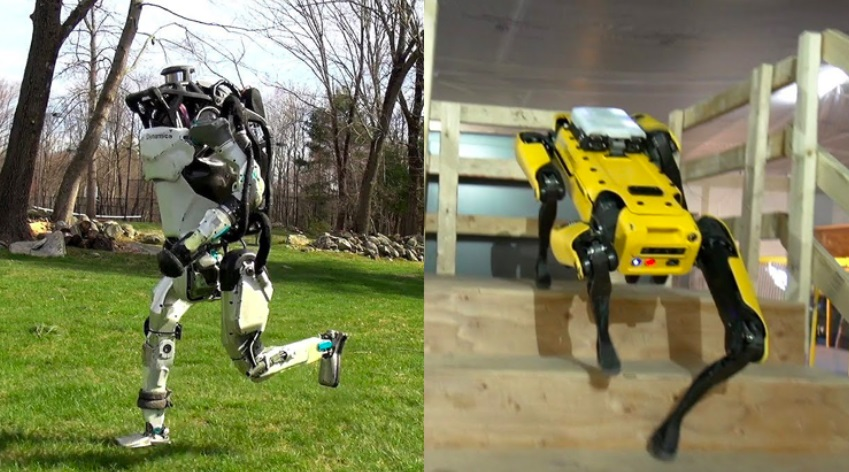
\includegraphics[width=.9\linewidth]{pic1.jpg}
  \captionof{figure}{Walking robots}
\end{minipage}%
\begin{minipage}{.5\textwidth}
  \centering
  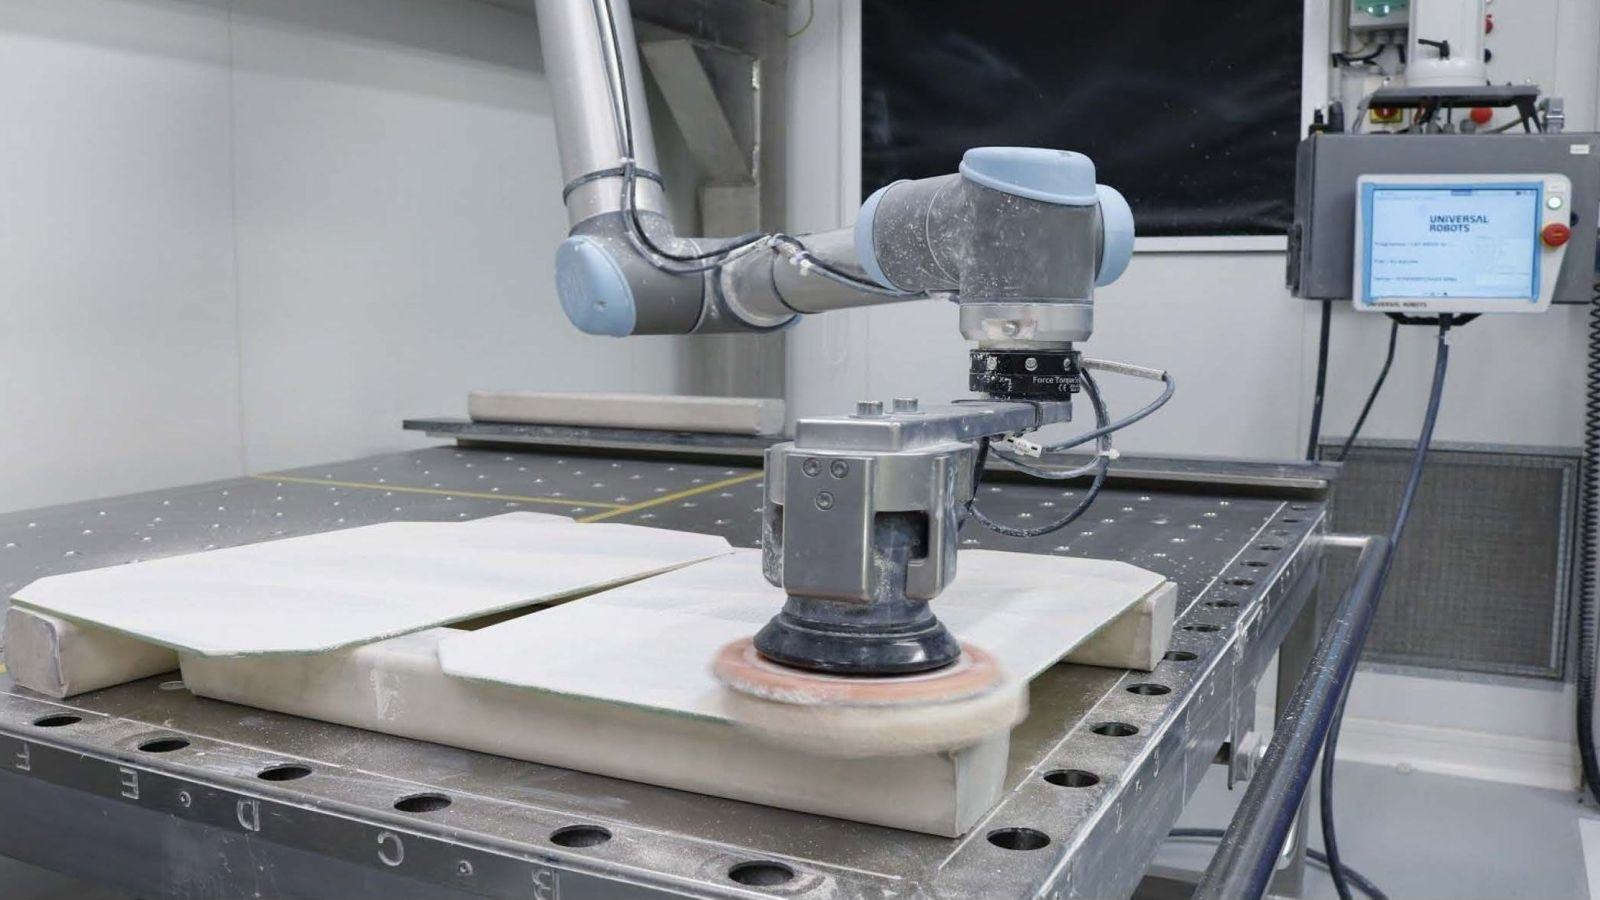
\includegraphics[width=.9\linewidth]{pic2.jpg}
  \captionof{figure}{Polishing with industrial arms}
\end{minipage}
\end{figure}

\end{flushleft}
\end{frame}




\begin{frame}{Typical reasons why explicit constraints arise}
% \framesubtitle{FF control of mechanical systems}
\begin{flushleft}

Explicit constraints are usually not a necessity and not a physical property of the problem. However, they are often encountered in practice. Typical situations when they are encountered as as follows:

\begin{itemize}
    \item Systems with contact interactions.
    \item Hybrid systems (two or more different dynamics which switch between one-another).
    \item Nonholonomic constraints in the dynamics (dynamics of a unicycle, bicycle, etc.).
    \item Dynamics is more clear and easy to work which when non-minimal representation is used.
\end{itemize}

\end{flushleft}
\end{frame}


\begin{frame}{Ways to control systems with explicit constraints}
% \framesubtitle{FF control of mechanical systems}
\begin{flushleft}

There are basic ways to deal with such systems:

\begin{itemize}
    \item Reduce to a system with implicit constraints and control that system instead.
    \item Treat reaction forces as a yet another external force.
    \item Design control law based on the explicit representation of constraints.
\end{itemize}

\end{flushleft}
\end{frame}



\begin{frame}{Constrained LTI}
% \framesubtitle{O}
\begin{flushleft}

Consider equations in the form:

\begin{equation}
\label{eq:LTI}
    \dot{\mathbf{x}} = \mathbf{A} \mathbf{x} + \mathbf{B} \mathbf{u} + \mathbf{c}
\end{equation}

where $\mathbf{A}$ is the state matrix, $\mathbf{B}$ is the control matrix and $\mathbf{c}$ is the affine term of the affine dynamics model.

\bigskip

For systems with constraints the same linearization takes form:

\begin{equation}
\label{eq:CLTI}
\begin{cases}
    \dot{\mathbf{x}} = \mathbf{A} \mathbf{x} + \mathbf{B} \mathbf{u} + \mathbf{S} \lambda + \mathbf{c} \\
    \mathbf{G}\dot{\mathbf{x}} = 0
\end{cases}    
\end{equation}

where $\mathbf{S}$ is linearized constraint Jacobian and $\mathbf{G} = \begin{bmatrix} \mathbf{F} & \mathbf{0} \\ \dot{\mathbf{F}} & \mathbf{F} \end{bmatrix}$. 

\end{flushleft}
\end{frame}



\begin{frame}{Minimal representation}
\framesubtitle{Part 1}
\begin{flushleft}

We can observe that constraint $\mathbf{G}\dot{\mathbf{x}} = 0$ implies that all feasible state velocities $\dot{\mathbf{x}}$ lie in the null space of $\mathbf{G}$. This means that we can introduce a new lower dimensional variable $\mathbf{z}$ to describe $\mathbf{x}$ (assuming initial value of $\mathbf{x}$ lies in the column space of $\mathbf{N}$):

\begin{equation}
    \mathbf{N}\mathbf{z} = \mathbf{x}
\end{equation}

where $\mathbf{N} = \text{null}(\mathbf{G})$ - orthonormal basis in the null space of $\mathbf{G}$. 
\end{flushleft}
\end{frame}


\begin{frame}{Minimal representation}
\framesubtitle{Part 2}
\begin{flushleft}

Let us re-express dynamics \eqref{eq:CLTI} in terms of $\mathbf{z}$ by multiplying it by $\mathbf{N}^\top$ on the left:

\begin{equation}
    \mathbf{N}^\top \dot{\mathbf{x}} = \mathbf{N}^\top \mathbf{A} \mathbf{x} + \mathbf{N}^\top \mathbf{B} \mathbf{u} + \mathbf{N}^\top \mathbf{S} \lambda + \mathbf{N}^\top \mathbf{c}
\end{equation}

We can prove that $\mathbf{N}^\top \mathbf{S} = 0$ for all mechanical systems (for example, by observing that mechanical constrains do not do work) or check that our particular $\mathbf{S}$ lies in the row space of our $\mathbf{G}$.

Noting that $\dot{\mathbf{z}} = \mathbf{N}^\top \dot{\mathbf{x}}$ and $\mathbf{x} = \mathbf{N}\mathbf{z}$ we get:

\begin{equation}
    \dot{\mathbf{z}} = \mathbf{N}^\top \mathbf{A} \mathbf{N} \mathbf{z} + \mathbf{N}^\top \mathbf{B} \mathbf{u} + \mathbf{N}^\top \mathbf{c}
\end{equation}

Defining $\mathbf{A}_N = \mathbf{N}^\top \mathbf{A} \mathbf{N}$, $\mathbf{B}_N = \mathbf{N}^\top \mathbf{B}$ and $\mathbf{c}_N = \mathbf{N}^\top \mathbf{c}$ we get:

\begin{equation}
    \dot{\mathbf{z}} = \mathbf{A}_N \mathbf{z} + \mathbf{B}_N \mathbf{u} + \mathbf{c}_N
\end{equation}

\end{flushleft}
\end{frame}




\begin{frame}{Minimal representation}
\framesubtitle{Part 3}
\begin{flushleft}

Since we achieved that our constrained dynamics is written in the standard LTI form:

\begin{equation}
    \dot{\mathbf{z}} = \mathbf{A}_N \mathbf{z} + \mathbf{B}_N \mathbf{u} + \mathbf{c}_N,
\end{equation}

we can use standard LTI control methods on it, for example finding optimal feedback gains via pole placement or LQR:

\begin{equation}
    \mathbf{K}_N = \text{lqr}(\mathbf{A}_N, \mathbf{B}_N, \mathbf{Q}, \mathbf{R})
\end{equation}

where $\mathbf{Q}$ and $\mathbf{R}$ are matrices defining cost function for the LQR problem.

\end{flushleft}
\end{frame}



\begin{frame}{Inverse dynamics}
\framesubtitle{LTI}
\begin{flushleft}

For any LTI system, including the LTI form of a constrained system we saw previously, inverse dynamics can be solved precisely by a pseudo-inverse, as long as there exist a solution. The following condition verifies it:

\begin{equation}
    (\mathbf{I} - \mathbf{B}\mathbf{B}^+)(\dot{\mathbf{x}} - \mathbf{A} \mathbf{x} - \mathbf{c}) = 0,
\end{equation}

The condition checks if vector $(\dot{\mathbf{x}} - \mathbf{A} \mathbf{x} - \mathbf{c})$ lies in the column space of $\mathbf{B}$. If it holds, precise solution to inverse kinematics can be found as:

\begin{equation}
    \mathbf{u}_{ID} = \mathbf{B}^+(\dot{\mathbf{x}} - \mathbf{A} \mathbf{x} - \mathbf{c}).
\end{equation}

\end{flushleft}
\end{frame}



\begin{frame}{Inverse dynamics}
\framesubtitle{Manipulator equations}
\begin{flushleft}

For a constrained mechanical system we can solve inverse dynamics without the need for linearization. Consider the following dynamics:

\begin{equation}
    \mathbf{H}\ddot{\mathbf{q}} + \mathbf{C}\dot{\mathbf{q}} + \mathbf{g} = \mathbf{T}\mathbf{u} + \mathbf{F}^\top \lambda
\end{equation}

We can represent constraint Jacobian $\mathbf{F}^\top$ as its QR decomposition: $\mathbf{F}^\top = \mathbf{Q} \begin{bmatrix} \mathbf{R} \\ \mathbf{0}  \end{bmatrix}$, where $\mathbf{Q}^\top \mathbf{Q} = \mathbf{Q} \mathbf{Q}^\top = \mathbf{I}$ and $\mathbf{R}$ is convertible.

\begin{equation}
    \mathbf{H}\ddot{\mathbf{q}} + \mathbf{C}\dot{\mathbf{q}} + \mathbf{g} = \mathbf{T}\mathbf{u} + \mathbf{Q} \begin{bmatrix} \mathbf{R} \\ \mathbf{0}  \end{bmatrix} \lambda
\end{equation}


\end{flushleft}
\end{frame}


\begin{frame}{Inverse dynamics}
\framesubtitle{Manipulator equations, part 2}
\begin{flushleft}

Let us multiply the equation by $\mathbf{Q}^\top$:

\begin{equation}
    \mathbf{Q}^\top (\mathbf{H}\ddot{\mathbf{q}} + \mathbf{Q}^\top\mathbf{C}\dot{\mathbf{q}} + \mathbf{g}) = \mathbf{Q}^\top\mathbf{T}\mathbf{u} + \begin{bmatrix} \mathbf{R} \\ \mathbf{0}  \end{bmatrix} \lambda
\end{equation}

Introducing switching variables (to divide upper and lower part of the equations) $\mathbf{S}_1 = \begin{bmatrix} \mathbf{I} & \mathbf{0}  \end{bmatrix}$ and $\mathbf{S}_2 = \begin{bmatrix} \mathbf{0} & \mathbf{I}  \end{bmatrix}$ and multiplying equations by one and the other we get two systems:

\begin{equation}
\begin{cases}
    \mathbf{S}_1 \mathbf{Q}^\top (\mathbf{H}\ddot{\mathbf{q}} + \mathbf{Q}^\top\mathbf{C}\dot{\mathbf{q}} + \mathbf{g}) = \mathbf{S}_1\mathbf{Q}^\top\mathbf{T}\mathbf{u} + \mathbf{R} \lambda \\
    \mathbf{S}_2 \mathbf{Q}^\top (\mathbf{H}\ddot{\mathbf{q}} + \mathbf{Q}^\top\mathbf{C}\dot{\mathbf{q}} + \mathbf{g}) = \mathbf{S}_2\mathbf{Q}^\top\mathbf{T}\mathbf{u}
\end{cases}
\end{equation}

The main advantage we achieved is that now we can calculate both $\mathbf{u}$ and $\lambda$

\end{flushleft}
\end{frame}


\begin{frame}{Inverse dynamics}
\framesubtitle{Manipulator equations, part 3}
\begin{flushleft}

Resulting expression for $\mathbf{u}$ is:

\begin{equation}
    \mathbf{u} = 
    (\mathbf{S}_2\mathbf{Q}^\top\mathbf{T})^+ \mathbf{S}_2 \mathbf{Q}^\top (\mathbf{H}\ddot{\mathbf{q}} + \mathbf{Q}^\top\mathbf{C}\dot{\mathbf{q}} + \mathbf{g})
\end{equation}

Expression for $\lambda$ is:

\begin{equation}
\lambda = \mathbf{R}^{-1} \mathbf{S}_1 \mathbf{Q}^\top (\mathbf{H}\ddot{\mathbf{q}} + \mathbf{Q}^\top\mathbf{C}\dot{\mathbf{q}} + \mathbf{g} - \mathbf{T}\mathbf{u})
\end{equation}

We can notice a pseudo-inverse, implying that the no-residual solution does not have to exist.

\end{flushleft}
\end{frame}



\begin{frame}{Inverse dynamics}
\framesubtitle{Quadratic program}
\begin{flushleft}

We can easily write inverse dynamics as a QP:


\begin{equation}
\begin{aligned}
& \underset{\mathbf{u}, \lambda}{\text{minimize}}
& & ||\mathbf{u}||, \\
& \text{subject to}
& & \begin{cases}
    \mathbf{H}\ddot{\mathbf{q}} + \mathbf{C}\dot{\mathbf{q}} + \mathbf{g} = \mathbf{T}\mathbf{u} + \mathbf{F}^\top \lambda \\
    \mathbf{F}\ddot{\mathbf{q}} + \dot{\mathbf{F}}\dot{\mathbf{q}} = 0
    \end{cases}
\end{aligned}
\end{equation}

If there are some constraints or limits on the control input (torque limits, for instance) or the reaction forces are restricted (by friction cones, for instance), those can be directly added.

\end{flushleft}
\end{frame}



\begin{frame}{Read more}

\begin{itemize}
\item Mason, S., Righetti, L. and Schaal, S., 2014, November. Full dynamics LQR control of a humanoid robot: An experimental study on balancing and squatting. In 2014 IEEE-RAS International Conference on Humanoid Robots (pp. 374-379). IEEE.

\item Mason, S., Rotella, N., Schaal, S. and Righetti, L., 2016, November. Balancing and walking using full dynamics LQR control with contact constraints. In 2016 IEEE-RAS 16th International Conference on Humanoid Robots (Humanoids) (pp. 63-68). IEEE. - \href{https://arxiv.org/pdf/1701.08179}{arxiv.org/pdf/1701.08179}

\item Mistry, M., Buchli, J. and Schaal, S., 2010, May. Inverse dynamics control of floating base systems using orthogonal decomposition. In 2010 IEEE international conference on robotics and automation (pp. 3406-3412). IEEE. - \href{http://citeseerx.ist.psu.edu/viewdoc/download?doi=10.1.1.212.3601&rep=rep1&type=pdf}{citeseerx.ist.psu.edu/viewdoc/download?doi=10.1.1.212.3601\&rep=rep1\&type=pdf}
\end{itemize}

\end{frame}




\begin{frame}{Thank you!}
\centerline{Lecture slides are available via Moodle.}
\bigskip
\centerline{You can help improve these slides at:}
\centerline{
\textcolor{blue}{\centerline{\href{https://github.com/SergeiSa/Control-Theory-Slides-Spring-2021}{github.com/SergeiSa/Control-Theory-Slides-Spring-2021}}}}

\bigskip

\textcolor{black}{\qrcode[height=1.5in]{github.com/SergeiSa/Control-Theory-Slides-Spring-2021}}

\bigskip

\centerline{Check Moodle for additional links, videos, textbook suggestions.}
\end{frame}

\end{document}
